\section{Gr"unde f"ur Analphabetismus} \label{sec:reasons}

Hier an dieser Stelle fragt man sich nat"urlich "'\textit{Wie kann es sein, dass so viele Menschen niemals Lesen und Schreiben gelernt haben?}"` Immerhin gibt es besonders in Deutschland die Schulpflicht, wo einem Lesen und Schreiben beigebracht wird. Wie kann es da also sein, dass ganze 6\% der deutschen Bev"olkerung Analphabeten sind? Hat das Bildungssystem versagt? \\


\subsection{Bildung}

Die Antworten auf die Frage wieso so viele Menschen in Deutschland Analphabeten sind, sind zum gro"sen Teil subtiler als man denken w"urde. Hier spielen zudem viele Faktoren eine Rolle wie Familie, Freunde und die einfache Mentalit"at eines Menschen. Um direkt ein kleines Beispiel f"ur den Bereich der Mentalit"at zu nennen, gehen wir zur"uck in die Anf"ange der Schulzeit. Dabei wollen wir folgenden Teil auf den Erfahrungsbericht eines Analphabeten stützen, welchen wir später noch genauer behandeln werden.
\footnoteSource {Sabine Kuhn-Behrenbeck}
				{Dumm bin ich weiß Gott nicht}
				{18.01.2013 }
				{http://www.mobile-elternmagazin.de/wireltern/partnerschaft_familie/details?k_onl_struktur=385577&k_beitrag=523759}
In diesem Erfahrungsbericht geht es um Bernd Dahler, welcher zu seiner Zeit eine schwierige Phase in der Schule hatte. Er war starker Stotterer und wenn er etwas vorlesen sollte in der Schule, wurde er von den anderen Kindern ausgelacht, weshalb er versuchte solche Situationen zu vermeiden. Außerdem ist Bernd Linkshänder und wurde von seinem Lehrer gezwungen mit der rechten Hand zu schreiben, weshalb es ihm zusätzlich noch schwerer gefallen ist. Als er im Anschluss die Grundschule verließ und auf die Hauptschule kam, mogelte Bernd sich nur noch durch. Wurden Klassenarbeiten geschrieben, blieb er zuhause und spielte krank. Viel vom Unterrichtsstoff bekam er mit und merkte sich alles auf seine eigene Weise. Er bestand die Hauptschule schließlich, erhielt allerdings von den Lehrern in seinem Zeugnis auch den Vermerk, dass er nicht lesen und schreiben kann.\\
All dies muss aber auch noch unter anderen Aspekten berücksichtigt werden.
Wie allgemein bekannt ist, lernen nicht alle Menschen im gleichen Tempo, weshalb einige mehr Zeit und mehr Aufmerksamkeit benötigen um ihre Aufgaben zu meistern. Wird denen, die langsamer lernen, die entsprechende Aufmerksamkeit in Bezug auf die Betreuung nicht gewährt, fallen sie zurück und schaffen es teils nicht den entsprechend "`verpassten"' nachzuholen, da sie versuchen sich mit an die neuen Themen anzuhängen und dabei schließlich gänzlich den Faden verlieren. Dies deutet allerdings keineswegs darauf hin, dass die entsprechenden Personen lernbehindert sind. Es zeigt sich eher, dass nicht alle Menschen auf die gleiche Art und Weise Dinge aufnehmen und Bezüge herstellen. Aus diesem Grund ist es eigentlich notwendig, dass verschiedene Lehrmethoden auf größere Gruppen angewendet werden.\\

Dieses Beispiel soll nur eine von vielen Möglichkeiten illustrieren, wieso so viele erwachsene Menschen in Ländern, in denen Schulpflicht herrscht Analphabeten sind. \\

Weitere sehr ernstzunehmende Probleme lassen sich bspw. mit Küstermanns Zitat vom Neuköllner Verein "'Lesen \& Schreiben e.V."' erläutern.


\begin{quote}
	"`Ein Hauptproblem ist, dass Muttersprachler gesetzlich
	kein Anrecht auf nachträglichen Schriftspracherwerb
	haben, anders als Bürger mit Migrationshintergrund. Hier
	gibt es bisher für Deutsche, die an den Rand der
	Gesellschaft gedrängt werden, kaum Angebote, die
	finanziert werden."'
\footnoteSource {Oliver Ohmann}
				{Zwei Berliner über ihr Leben ohne Worte}
				{02.02.2013}
				{http://www.bz-berlin.de/aktuell/berlin/zwei-berliner-ueber-ihr-leben-ohne-worte-article1133404.html}
\end{quote}


Zu dem sollte noch erwähnt werden, wie Analphabeten heute in etwa auf das Bildungssystem abgebildet werden können.\\
Nach Studien - die wir leider nicht nachprüfen konnten, aber dennoch erwähnen möchten - haben etwa 

\begin{itemize}
	\item 19\% der Analphabeten keinen Schulabschluss
	\item 48\% erreichten einen Hauptschulabschluss
	\item 19\% haben einen Realschulabschluss
	\item und 12\% erreichten sogar einen höheren Schulabschluss wie das Abitur
\end{itemize}

Leider wurden die hier fehlenden 2\% nicht weiter erwähnt.
\footnoteSource {Prof. Dr. Anke Grotlüschen, Dr. Wibke Riekmann}
				{Ein Mensch wie Du und ich}
				{02.06.2013}
				{http://blogs.epb.uni-hamburg.de/leo/files/2012/09/2012-19-10-leo-f\%C3\%BCr-Fachtagung-Bad-Wildungen.pdf.}



\subsection{Legasthenie}

Legasthenie ist eine Erbkrankheit, bei der eine Störung der visuellen und auditiven Wahrnehmungsverarbeitung auftritt. Menschen mit dieser Störung leiden nicht an mangelndem Intellekt oder an motorischen Einschränkungen, stattdessen ist einfach ihr Sehen und/oder ihr Hören beeinträchtigt. Dadurch können diese Menschen Text nicht richtig entziffern und können auch gesprochene Worte einfach akustisch nicht richtig verstehen. Experten sind sich uneinig, ob Legasthenie heilbar ist, oder nicht, was auf diverse Quellen mit verschiedenen Meinungen zurückzuführen ist.
\footnoteSource{Prof. Dr. Renate Valtin, Dr. Ilona Löffler}
				{Legasthenie ist heilbar}
				{02.06.2013}
				{http://www.dgls.de/download/category/4-tagungen.html?download=44:r-valtin-und-i-loeffler-legasthenie-ist-heilbar}
\footnoteSource{Andrea Schultens}
				{Wie unterscheiden sich Analphabetismus und Legasthenie?}
				{02.06.2013}
				{http://www.planet-wissen.de/alltag_gesundheit/lernen/analphabeten/wissensfrage.jsp}
 In jedem Falle wird bei einer frühzeitigen Diagnose dazu geraten, das Kind einem speziellen Training zu unterziehen, damit es die sehenden und akustischen Eigenschaften, die nicht richtig ausgebildet sind, nach entwickelt. Um ein näheres Gefühl und Verständnis dafür zu bekommen, wieso ein Legastheniker solch enorme Schwierigkeiten hat Text zu erkennen und zu entziffern, soll folgende Grafk dienen.\\

\begin{figure}[h]
	\centering
		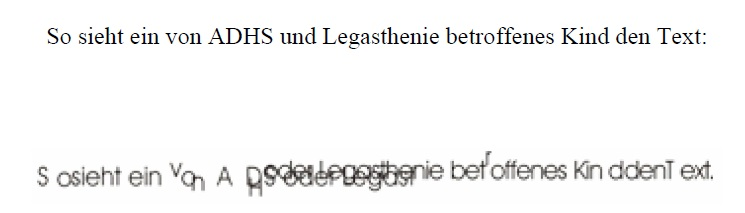
\includegraphics[width=1.00\textwidth]{Daten/legastheneWahrnehmung.jpg}
	\caption{Legasthene Wahrnehmung}
	\url{http://www.landeselternrat-sachsen.de/fileadmin/ler/daten/01ler/04sitzungen/92--06-07_07-08/080419_Vortrag-Bock.pdf}
	\label{fig:legastheneWahrnehmung}
\end{figure}